%! Author = Filippo Vissani
%! Date = 08/02/24
% !TeX root = ../thesis-main.tex

%----------------------------------------------------------------------------------------
\chapter{Validation}
\label{chap:evaluation}
%----------------------------------------------------------------------------------------

This chapter delves into the evaluation of the reactive extensions introduced into the Collektive framework. The chapter is divided into two main sections:

\begin{itemize}
    \item \Cref{section:testing} details the unit testing strategy employed to ensure the correctness of the implemented code. It highlights the chosen testing framework, and the testing style adopted, and showcases an example test related to the \texttt{rExchange} construct.
    \item \Cref{section:analysis-ergonomics-proposed-models} compares the usability of the \ac{dsl} for implementing aggregate programs in the two proposed reactive models. To facilitate the comparison, an example program implementing the "gradient with obstacles" scenario is presented in both DSLs. This allows for a concrete side-by-side assessment of the strengths and weaknesses of each model from a usability perspective.
\end{itemize}

\section{Testing}
\label{section:testing}

Ensuring the correctness of the implemented reactive extensions is paramount to their successful integration within the Collektive framework. This section delves into the testing strategies employed, focusing on unit testing methodologies.

The project adopts a rigorous approach to testing, leveraging the Kotest framework for automated testing in Kotlin. Kotest\footnote{\url{https://kotest.io/}.} provides a robust testing environment conducive to comprehensive test suites. Among its testing styles, the project opted for \texttt{StringSpec} due to its straightforward structure, which facilitates a behavior-driven approach to test composition. The most relevant tests within the project are those that verify the behavior of the aggregate constructs.

Unit tests are designed to verify the behavior of the aggregate constructs, ensuring they function as expected across various scenarios. Tests are crafted to cover different aspects of the reactive functionality, ensuring the accurate alignment of devices and the correctness of values exchanged and validating the correctness of aggregate expressions and resultant values.

An example test case for the \texttt{rExchange} construct is presented in \Cref{lst:rexchange-test} to illustrate the testing approach. The test case encompasses the following steps:

\begin{enumerate}
    \item Definition of the test name and sequential execution within a coroutine.
    \item Definition of the aggregate result based on the execution of the aggregate program in a specific aggregate context.
    \item Launching a concurrent job to execute the simulation.
    \item Introduction of a delay and subsequent cancellation of the job.
    \item Assertion of the expected results against the computed values.
\end{enumerate}

The provided example test serves as a template for testing other reactive constructs, ensuring thorough validation of their behavior.

\lstinputlisting[float,language=kotlin,label={lst:rexchange-test},caption=Part of the test suite related to the \texttt{rExchange} construct.]{listings/rexchange-test.kt}

\section{Analysis of the Ergonomics of the Proposed Models}
\label{section:analysis-ergonomics-proposed-models}

This section evaluates the usability and effectiveness of the proposed reactive models within the Collektive framework. The evaluation focuses on readability, maintainability, flexibility, and the learning curve associated with each model.

The aggregate program chosen to carry out this evaluation is the gradient with obstacles, which maintains the properties of the classic gradient, but introduces obstacles into the environment. \Cref{fig:gradient-environment-and-execution} shows a graphical representation of what you want to achieve. There are three types of nodes in the environment: sources (green), obstacles (red) and defaults (blue). The objective is to calculate the distance of each node from the nearest source without considering the neighbors who are considered as obstacles. The environment used in this case is a grid with five columns and five rows, where each device is a neighbor of the nearest device in each horizontal and vertical direction. In addition, the device with ID 0 is a source node, while devices with ID 2, 7, and 12 are obstacles.

\Cref{lst:gradient-obstacles-prm} and \Cref{lst:gradient-obstacles-rmsm} present the implementation of the gradient with obstacles in the purely reactive model and in the one where only sensors and messages are reactive, respectively. In both cases the node type is defined as \texttt{StateFlow<NodeType>}, allowing to change sources and obstacles at runtime. What changes is how this flow is managed: in the purely reactive case it is used directly within the aggregate constructs, while in the other a specific simulator must be created, which reevaluates the expression as the type of node varies. As regards the use of aggregate constructs within the program, the model with reactive messages and sensors is equivalent to the proactive model, while in the purely reactive model, the use of functions for manipulating flows introduces greater complexity. Based on the results obtained, the following considerations arise:


\paragraph{Readability}

In the purely reactive model, the use of rShare, rMux, and rBranch might be less familiar to developers unfamiliar with this specific \ac{dsl}. Understanding the syntax and purpose of these functions requires additional learning. The model with reactive messages and sensors utilizes familiar syntax like share and conditional statements, potentially making it easier to read and understand for developers with general programming experience.

\paragraph{Maintainability}

Composing complex logic using nested functions like rMux and rBranch can lead to nested code structures, potentially impacting maintainability as the codebase grows. In the model with reactive messages and sensors conditional statements and function calls promote a more linear and explicit flow of logic, potentially improving maintainability.

\paragraph{Flexibility}

The \ac{dsl} of the purely reactive model provides dedicated functions for building reactive constructs, potentially offering more flexibility for complex reactive patterns. While offering less specialized syntax, the model with reactive messages and sensors can still achieve various reactive behaviors. However, complex reactive patterns might require more verbose code compared to the purely reactive approach.

\paragraph{Learning Curve}

The purely reactive model requires learning the specific syntax and semantics of the \ac{dsl} functions, while the model with reactive messages and sensors leverages familiar programming constructs, potentially reducing the learning curve for developers with general programming experience.

\begin{figure}
    \centering
    \begin{subfigure}[b]{.15\textwidth}
        \centering
        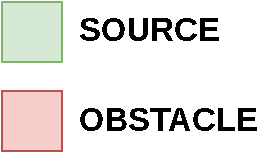
\includegraphics[width=\textwidth]{figures/gradient-environment-legend.pdf}
        \label{fig:gradient-legend}
    \end{subfigure}
    \hfill
    \begin{subfigure}[b]{.49\textwidth}
        \centering
        
\includegraphics[width=\textwidth]{figures/palette-cropped2.png}
        \label{fig:gradient-palette}
    \end{subfigure}
    \hfill
    \begin{subfigure}[b]{.49\textwidth}
        \centering
        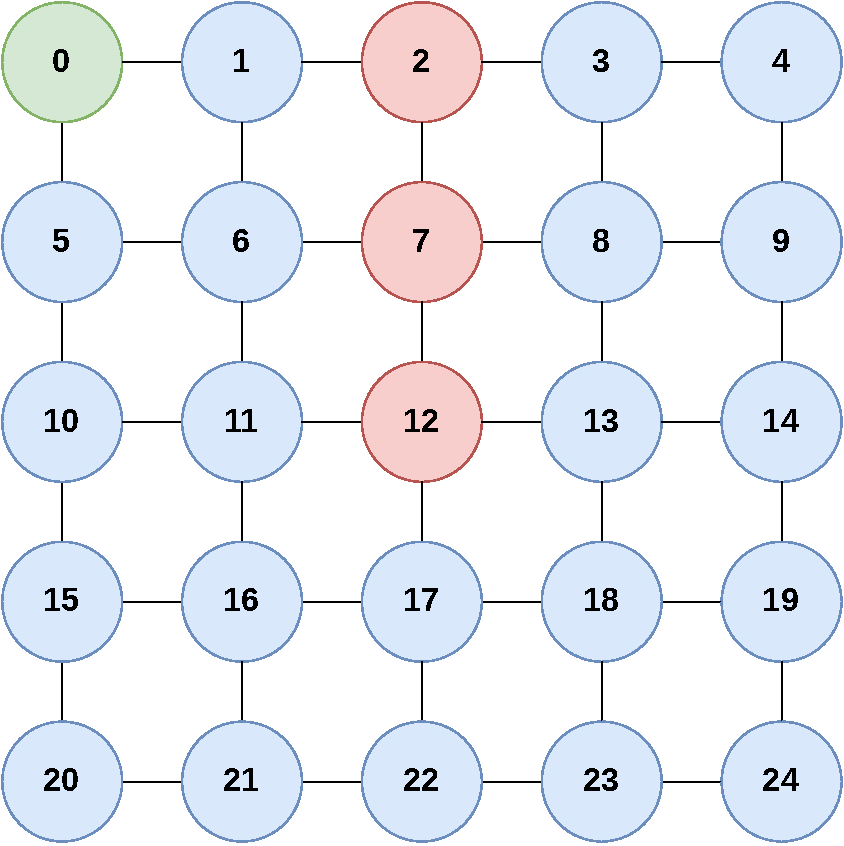
\includegraphics[width=\textwidth]{figures/gradient-environment.pdf}
        \caption{}
        \label{fig:gradient-envronment}
    \end{subfigure}
    \hfill
    \begin{subfigure}[b]{.49\textwidth}
        \centering
        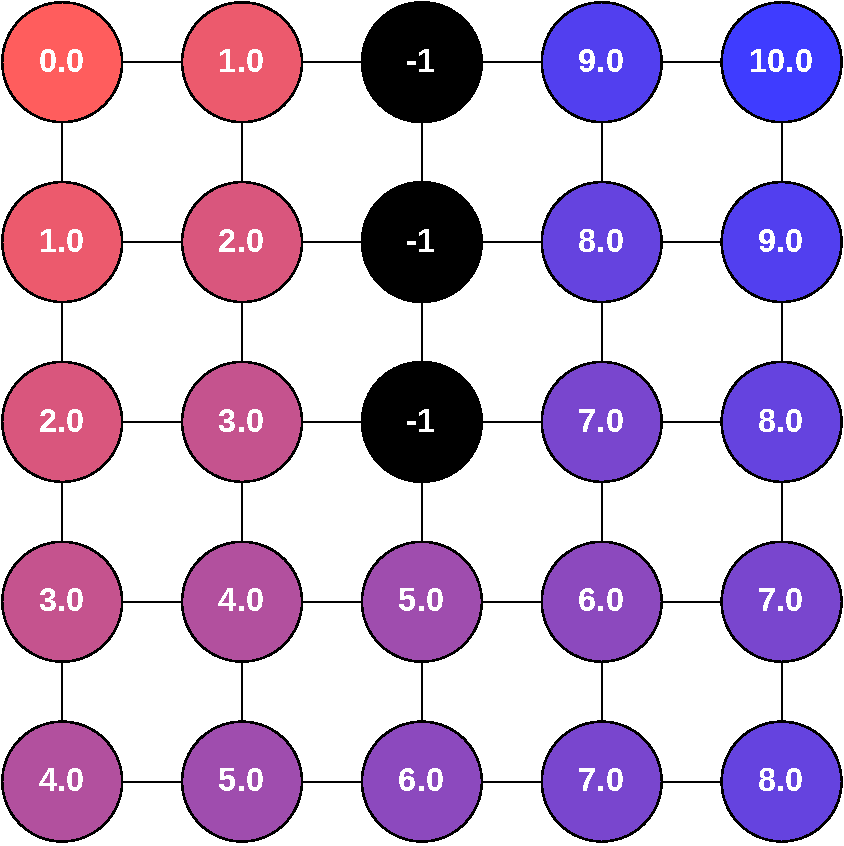
\includegraphics[width=\textwidth]{figures/gradient-environment-execution.pdf}
        \caption{}
        \label{fig:gradient-envronment-execution}
    \end{subfigure}
    \caption{\Cref{fig:gradient-envronment} presents the environment where the gradient with obstacles was executed. The node highlighted in green represents the source, while those in red represent the obstacles. \Cref{fig:gradient-envronment-execution} presents the output field of the gradient with obstacles after stabilization.}
    \label{fig:gradient-environment-and-execution}
\end{figure}

\lstinputlisting[float,language=kotlin,label={lst:gradient-obstacles-prm},caption=Gradient with obstacles implementation in purely reactive model.]{listings/gradient-obstacles-prm.kt}

\lstinputlisting[float,language=kotlin,label={lst:gradient-obstacles-rmsm},caption=Gradient with obstacles implementation in model with reactive messages and sensors.]{listings/gradient-obstacles-rmsm.kt}
